
%%%%%%%%%%%%%%%%%%%%%%%%%%%%%%%%%%%%%%%%%%%%%%%%%%%%%%%%%%%%%
%
% Section: Linear Functions and Their Graphs
%
%%%%%%%%%%%%%%%%%%%%%%%%%%%%%%%%%%%%%%%%%%%%%%%%%%%%%%%%%%%%

\section{Linear Functions and Their Graphs}
\label{LinearFunctionsGraphs}

We have already discussed the graphs of linear functions in the previous sections of this chapter.\\

Some key points that we have noted:

\begin{itemize}
	\item The graphs of linear functions are straight lines
	\item The slope can be interpreted as $\frac{rise}{run}$ and determines the steepness of the line
	\item The vertical intercept is where the graph crosses the vertical axis
\end{itemize}

In this section we will discuss some other facts about linear functions’ graphs, and the uses to which they can be put.

%%%%%%%%%%%%%%%%%%%%%%%%%%%%%%%%%%%%%%%%%%%%%%%%%%%%%%%%%%%%%
%
% Section: Linear Functions and Their Graphs: Graphical Solution of Linear Equations
%
%%%%%%%%%%%%%%%%%%%%%%%%%%%%%%%%%%%%%%%%%%%%%%%%%%%%%%%%%%%%

\subsection{Graphical Solution of Linear Equations}

When working with linear mathematical models, we often need to solve equations that arise from linear functions. Not surprisingly, these equations are called linear equations.\\

It is often simplest to solve linear equations using regular run-of-the-mill algebra. However, graphical solution is also an option. In the following example we will illustrate the use of graphical
solution for linear equations. You may want to review Section \ref{SolvingEquationsGraphically}, Solving Equations Graphically for a refresher.

\exam{\label{LinearFunctionsGraphsExample1} Menauhant Publishing Company has a contract that costs them a straight $\$80$ per hour for computer support over the phone. They are considering switching to a new contract that would require them to pay an annual fee of $\$3,000$ regardless of how much service they use, but they would then only be charged $\$50$ per hour. If they don’t need many hours of support, the old plan would be cheaper, since even though they’d pay a higher rate per hour they’d avoid the $\$3,000$ flat fee. On the other hand, if they use a lot of hours, it would be worth it to pay that fee to get the lower rate. How many hours of support would they need to use to break even between the two plans?
}

\indenttext{
	Under the current plan, the total cost is a linear function of hours: $f(x)=80x$.\\
	Under the new plan, the total cost would also be a linear function of hours: $g(x)=50x+3000$.\\
	\newline
	We are looking for the number of hours where the costs would be the same, so we need to solve the equation:
	$$80x=50x+3000$$
	To solve this equation graphically, we set \quotes{Y1=80X} and \quotes{Y2=50X+3000} and graph the results. With a little playing around to find an appropriate window, we get a graph that looks like this:
	\begin{figure}[H]
		\centering
		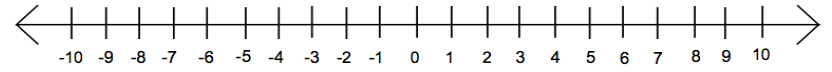
\includegraphics[scale=1.0]{sections/LinearFunctionsGraphsImages/Figure01.png}
		\caption{Graph of $f(x)=80x$ and $g(x)=50x+3000$}
	\end{figure}
	\noindent Running through the calculator Intersect program, we end up with the intersection X=$100$ and Y=$8000$. So, the break even point is $100$ hours of computer support.
}

\bigskip

In this first example, it probably would have been easier to just solve the equation with ordinary algebra. However, as we saw in Section \ref{SolvingEquationsGraphically}, with more complex equations graphical solution starts to become a more attractive option.  Which solution method you use in any given situation is to some degree at least a matter of personal preference - and it is always good to have a choice.

\exam{\label{LinearFunctionsGraphsExample2} Solve:  $$1.43x-2.07(1.08x-2.75)=3.12+2.59(0.76x-3.55)$$}

\indenttext{This is actually a linear equation; we can see that if we were to simplify each side them both sides could be put into slope-intercept form. We don’t need to actually do this though.\\
	\newline
	Graphing Y1=1.43X–2.07(1.08X–2.75) and Y2=3.12+2.59(0.76X-3.55) in the standard window we get:
	\begin{figure}[H]
		\centering
		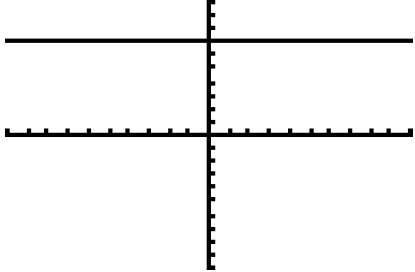
\includegraphics[scale=1.0]{sections/LinearFunctionsGraphsImages/Figure02.png}
		\caption{Graph in standard window.}
	\end{figure}
	\noindent The intersection gives us the solution: $x=4.24$ (rounded to two decimal places.)
}

%%%%%%%%%%%%%%%%%%%%%%%%%%%%%%%%%%%%%%%%%%%%%%%%%%%%%%%%%%%%%
%
% Subsection: Linear Functions and Their Graphs: Graphical Solution of Linear Inequalities
%
%%%%%%%%%%%%%%%%%%%%%%%%%%%%%%%%%%%%%%%%%%%%%%%%%%%%%%%%%%%%

\subsection{Graphical Solution of Linear Inequalities}

Sometimes we need to exactly match a particular goal, but often we really need to fall above or below a particular target. In those cases it is not an equation we need to solve, but instead an
inequality.\\

Graphing can be a very effective method for solving inequalities. To solve an inequality graphically, we follow the same process as we would use to solve an equation graphically. However, with the
inequality we want one side to be either below or above the other. So, we find the point where the two graphs cross (i.e. we find the intersection), and then choose the side of that intersection where
the graph of the side which is supposed to be less is below the side which is supposed to be more.\\

Consider the following reworking of the first example of this section:

\exam{\label{LinearFunctionsGraphsExample3} Menauhant Publishing Company has a contract that costs them a straight $\$80$ per hour for computer support over the phone. They are considering switching to a new contract that would require them to pay an annual fee of $\$3,000$ regardless of how much service they use, but they would then only be charged $\$50$ per hour. How many hours of support would they need to use for the new plan to be cheaper?
}

\indenttext{Here we are not trying to find the break-even point (where the old plan and new plan cost the same), we instead want the new plan to be cheaper. Since the new plan’s cost is $50x+3000$ and the old plan is $80x$, we need to solve: $$50x+3000=80x$$
	%In Chapter 1 we reviewed ways to solve inequalities like this one algebraically, but here we will
	Here we will solve it graphically. Letting Y1 be the left side and Y2 be the right side, we get the graph:
	\begin{figure}[H]
		\centering
		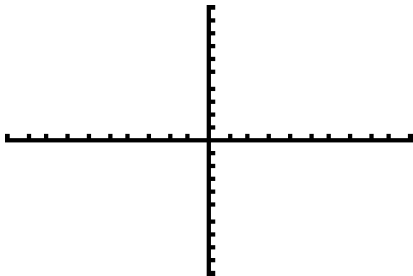
\includegraphics[scale=1.0]{sections/LinearFunctionsGraphsImages/Figure03.png}
		\caption{Graph of $f(x)=80x$ and $g(X)=50x+3000$}
	\end{figure}
	\noindent The two lines intersect at $x=100$ but this time we are interested in what happens before and after that intersection as well. We know that Y1, old new plan, has a smaller slope than Y2, the new
	plan, so Y1 is the less-steep line. Now, since we want Y1 the new plan to be less than Y2, the old plan, we want the less-steep line to be below the more-steep one. We can see from the graph that
	this happens to the right of the intersection – so our inequality is satisfied whenever $x>100$. (We do not include the intersection itself in our solution since the problem stated that we wanted the
	new plan to be strictly cheaper than the old plan, and at $100$ hours the two plans are equal.) So we conclude that this is our solution: the new plan will be cheaper if the company uses more than
	$100$ hours of computer support.
}

\bigskip

In this example we could readily tell which graph represented which side simply by looking at the steepness and slope. When finding the slope would require some algebraic effort, though, there is another approach.

\exam{\label{LinearFunctionsGraphsExample4} Solve: $$1.43x-2.07(1.08x-2.75) \geq 3.12+2.59(0.76x-3.55)$$}

\indenttext{This inequality has the same two sides as the equation we solved in Example \ref{LinearFunctionsGraphsExample2}, so the graph will be the same. Because neither side was in slope-intercept form, though, the slopes are not obvious, so we can’t use the slopes to determine which line belongs to which side. We could work them out by putting each side into slope-intercept form, but it is not really necessary for us to do this. If we hit the TRACE key on the calculator, the calculator will place the blinking TRACE icon on one of the graphs (usually Y1) and indicate which graph you are on at the top of the screen. The result should look like this:
	\begin{figure}[H]
		\centering
		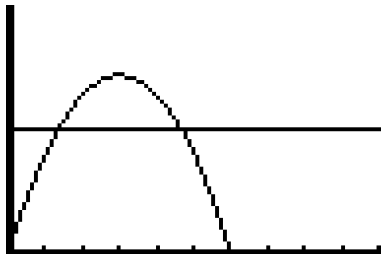
\includegraphics[scale=1.0]{sections/LinearFunctionsGraphsImages/Figure04.png}
		\caption{Graph showing TRACE}
	\end{figure}
	\noindent So now we can easily tell which side is Y1. Since we wanted Y1, the left side of the inequality, to be greater than or equal to Y2, the right, the solution to our inequality is the intersection and everything to the right of it, since Y1 is above Y2 to the right of the intersection. So the solution would be $x \leq 4.24$, or $\{x|x \leq 4.24\}$ or $(- \infty, 4.24]$. Note that since the original inequality was $\geq$ we include the intersection in our solution.
}

%%%%%%%%%%%%%%%%%%%%%%%%%%%%%%%%%%%%%%%%%%%%%%%%%%%%%%%%%%%%%
%
% Subsection: Linear Functions and Their Graphs: Parallel and Perpendicular Lines
%
%%%%%%%%%%%%%%%%%%%%%%%%%%%%%%%%%%%%%%%%%%%%%%%%%%%%%%%%%%%%

\subsection{Parallel and Perpendicular Lines}

We’ve already seen that sometimes equations don’t have any solutions. For example, if we try to solve: $$3x+7=3(x+1)$$
we distribute on the right: 

$$3x+7=3x+3$$

and then subtract $3x$ from both sides to get the obvious contradiction:  $$7=3$$ and so we conclude that this equation has no solutions.\\

Now, notice here that this is a linear equation; both sides of this equation can be regarded as linear functions. Looking at them that way, there is another way to see why this equation has no solutions. Both sides of this equation are lines with slope of 3. So they both have the same steepness. The one on the left crosses the vertical axis at 7, the other crosses the axis at 3 - so they are apart there, and since they rise with exactly the same steepness, they stay apart.\\

In other words, these lines are parallel. And following the logic above, we can see that two lines will be parallel whenever they have the same slopes. This is worth noting in general:

\begin{definition}
	\index{Linear Function!Parallel}
	\underline{Slopes of Parallel Lines}\\
	\bigskip
	Two lines are parallel if, and only if, they have the same slopes.
\end{definition}

We can use this fact to solve problems like the following.

\exam{\label{LinearFunctionsGraphsExample5} Find the formula for the linear function whose graph passes through the point $(-2,5)$ and is parallel to the graph of $f(x)=2x-3$.}

\indenttext{The slope of $f(x)=2x-3$ is 2. So our function must also have that slope. So we need to find the equation of the linear function with slope 2 and (-2,5) as an input-output pair.\\
	So:
	$$g(x)=2x+b\\5=2(-2)+b\\b=9$$
	And so we conclude that our function is $g(x)=2x+9$}

\bigskip

Sometimes we also have uses for lines that are perpendicular (that intersect in a right angle.) There is a relationship between their slopes as well. If two lines are perpendicular, if the one is rising, the other must be falling, and vice versa. So, their slopes must have opposite signs.\\

Also, two lines will be perpendicular if and only if they are \quotes{switching} their rises and runs. If the one rises three and runs one, the other must fall one and run three to make the intersection a right angle. And so:

\begin{definition}
	\index{Linear Function!Perpendicular}
	\underline{Slope of Perpendicular Lines}\\
	\bigskip
	Two lines are perpendicular if, and only if, they have opposite-signed reciprocal slopes.
\end{definition}

The following example will illustrate how this can be put to use.

\exam{\label{LinearFunctionsGraphsExample6} Find the formula for the linear function whose graph passes through the point $(3,-1)$ and is perpendicular to the graph of $f(x)=6x+11$.}

\indenttext{The slope of $f(x)=6x+11$ is $6$. So our function’s slope must be $-\frac{1}{6}$ since that is the opposite signed reciprocal. Continuing using the given input-output pair:
	$$g(x)=-\frac{1}{6}x+b\\ \\-1=-\frac{1}{6}(3)+b\\ \\b=-\frac{1}{2}$$
	So our function must be $g(x)=-\frac{1}{6}x-\frac{1}{2}$
}

%%%%%%%%%%%%%%%%%%%%%%%%%%%%%%%%%%%%%%%%%%%%%%%%%%%%%%%%%%%%
%
% Subsection: Linear Functions Graphs: Exercises
%
%%%%%%%%%%%%%%%%%%%%%%%%%%%%%%%%%%%%%%%%%%%%%%%%%%%%%%%%%%%%

\clearpage
\subsection{Exercises}

\subsubsection*{Graphical Solution of Linear Equations}

Round to two decimal places when necessary.

\bigskip
\ex{AAAwesome Car Rentals charges $\$17.50$ to rent a subcompact car for a day, plus $\$0.20$ per mile. BBBetter Auto Rents charges $\$25.00$ to rent a similar car for a day, plus $\$0.12$ per mile. How many miles would you have to drive for the two agency’s total costs to come out the same?}
\sol{$93.75$ miles}

\bigskip
\ex{To print a textbook, a printer charges a flat $\$5.75$ regardless of its length, plus a charge of $\$0.02$ per page. A competing printer charges $\$8.00$ plus $\$0.015$ per page. How many pages would a textbook need to be for the two printers’ costs to be the same?}

\bigskip
\ex{A car is doing $70$ mph when the driver begins to apply the brakes steadily, decreasing the speed by $0.5$ mph per second. When does the car’s speed reach $55$ mph?}
\sol{$30$ seconds}

\bigskip
\ex{I am driving from Rochester NY to Boston MA, a distance of $420$ miles. Assuming that I drive at a steady rate of exactly $60$ miles per hour, how long will it take before I reach Utica, which is
	$150$ miles from Rochester?}

\bigskip
\ex{Solve graphically: $4.24x - 1.03(2.02x - 1.79) = 4.24x + 1.03(2.02x - 1.79)$}
\sol{$x=0.89$}

\bigskip
\ex{Solve graphically: $1.07x - 4.12(3.02 - 1.17x) = 5.02 - 4.43x$}

\bigskip
\ex{Solve graphically: $300 - 25x = 250 + 10x$}
\sol{$x=1.43$}

\bigskip
\ex{Solve graphically: $100 + 25(x - 1) = 180 - 30x$}

\subsubsection*{Graphical Solution of Linear Inequalities}

Round to two decimal places when necessary.

\bigskip
\ex{AAAwesome Car Rentals charges $\$17.50$ to rent a subcompact car for a day, plus $\$0.20$ per mile. BBBetter Auto Rents charges $\$25.00$ to rent a similar car for a day, plus $\$0.12$ per mile.
	How many miles would you have to drive for AAAwesome to be the less expensive option?}
\sol{less than $93.75$ miles}

\bigskip
\ex{To print a textbook, a printer charges a flat $\$5.75$ regardless of its length, plus a charge of $\$0.02$ per page. A competing printer charges $\$8.00$ plus $\$0.015$ per page.  How many pages
	would a textbook need to be for the competing printers’ costs to be lower?}

\bigskip
\ex{A car is doing $70$ mph when the driver begins to apply the brakes steadily, decreasing the speed by $0.5$ mph per second. For how long is the car going faster than $55$ mph?}
\sol{for the first $30$ seconds}
	
\bigskip
\ex{I am driving from Rochester NY to Boston MA, a distance of $420$ miles. Assuming that I drive at a steady rate of exactly $60$ miles per hour, how long after I have reached Utica, which is
$150$ miles from Rochester, will I reach Boston?}
	
\bigskip
\ex{Solve graphically: $4.24x - 1.03(2.02x - 1.79) > 4.24x + 1.03(2.02x - 1.79)$}
\sol{$x<0.89$}
	
\bigskip
\ex{Solve graphically: $1.07x - 4.12(3.02 - 1.17x) > 5.02 - 4.43x$}

\bigskip
\ex{Solve graphically: $300 - 25x \leq 250 + 10x$}
\sol{$x \geq 1.43$}
	
\bigskip
\ex{Solve graphically: $100 + 25(x - 1) \geq 180 - 30x$}

\subsubsection*{Parallel and Perpendicular Lines}
	
\bigskip
\ex{Find the formula for the linear function whose graph passes through $(3,2)$ and whose graph is parallel to the graph of $f(x) = 2x - 9$.}
\sol{$g(x)=2x-4$}
	
\bigskip
\ex{Find the formula for the linear function whose graph passes through $(-2, -5)$ and whose graph is parallel to the graph of $f(x) = -3x + 1$.}
	
\bigskip
\ex{Find the formula for the linear function whose graph passes through $(-\frac{1}{2}, -\frac{3}{8})$ and whose graph is parallel to the graph of $f(x) = \frac{3}{4}x - \frac{19}{7}$.}
\sol{$g(x)=\frac{3}{4}x$}
	
\bigskip
\ex{Find the formula for the linear function whose graph passes through $(3,2)$ and whose graph is perpendicular to the graph of $f(x) = 2x - 9$.}
	
\bigskip
\ex{Find the formula for the linear function whose graph passes through $(-2, -5)$ and whose graph is perpendicular to the graph of $f(x) = -3x + 1$.}
\sol{$g(x)\frac{1}{3}-\frac{13}{3}$}
	
\bigskip
\ex{Find the formula for the linear function whose graph passes through $(-\frac{1}{2}, -\frac{3}{8})$ and whose graph is perpendicular to the graph of $f(x) = \frac{3}{4}x - \frac{19}{7}$.}
	
\subsubsection*{Grab Bag}
	
\bigskip
\ex{\begin{enumerate}[label=(\alph*)]
	\item Find the equation for the linear function whose graph is a line passing through $(-1,3)$ and which is parallel to the line $y = 3x - 4$.
	\item Find the equation for the linear function whose graph is a line passing through $(0,2)$ and which is perpendicular to the line $y = \frac{1}{2}x + \frac{43}{15}$. 
	\item Find the point where your answers to (a) and (b) intersect.
\end{enumerate}
}
\sol{a.  $g(x)=3x+6$\\  b.  $h(x)=2x+2$\\c.  $x=-4$}
	
\bigskip
\ex{A diagram drawn on a grid in a computer drafting program follows the graph of $f(x) = 2x - 9$. The program needs to display a line perpendicular to this line, passing through the point $(3, -3)$. Find a formula for this line.}
	
\bigskip
\ex{Jack has made $23$ dozen Christmas cookies so far and is making more at a steady rate of $5$ dozen per hour. Jill has made $11$ dozen and is making more at a rate of $9$ dozen per hour. Assuming they both continue at this same pace, when will they both have the same number of cookies?}
\sol{$3$ hours from now}
	
\bigskip
\ex{Solve for $t$: $4.3 - 1.08(2.45t - 1.35) \leq 11.1t - 3.25(2.75t - 0.64)$. Round to two decimal places if necessary.}
	
\bigskip
\ex{Solve for $x$. Round to two decimal places if necessary. $3.55x - 2.39(x - 1.17) = 5.02 - 2.93(1.15 - 0.93x)$.}
\sol{$x=0.73$}
	
\bigskip
\ex{Find equations for functions passing through the origin (a) parallel to $f(x) = -\frac{1}{2}x - 3$ and (b) perpendicular to $f(x) = -\frac{1}{2}x - 3$.}
	
\bigskip
\ex{I need to draw a line on a diagram perpendicular to the line $y = \frac{3}{2}x - 5$. The diagram is on a grid, and so I can count units of rise and run from my starting point to make sure that my line has the appropriate slope. What should the rise be? What should the run be?}
\sol{rise: $-2$, run: $+3$ OR rise: $+2$, run: $-3$}
	
\bigskip
\ex{I walk at a steady rate of $3.5$ miles per hour, and my friend walks at a rate of $2.7$	 miles per hour. We are both walking in the same direction, but she had a 1 mile head start. When will I
		catch up with her? }
	
\bigskip
\ex{A manufacturer can produce widgets at either of two factories. The time required to fill the order is a function of the number of crates of widgets ordered. At the first factory, filling an order
		requires $65$ minutes of setup time, plus $5$ minutes per crate of widgets ordered. The second factory requires only $40$ minutes of setup time, but takes $10$ minutes per crate. Under what circumstances would the first factory be require less time to fill an order?}
\sol{if the order is for more than $5$ crates}
	
\bigskip
\ex{Solve for $z$ rounded to two decimal places if necessary: $\frac{2.46z-1.13}{0.65} = 5.12 - 0.11(13.29z - 0.41)$.}
	
\bigskip
\ex{Solve for $z$ rounded to two decimal places if necessary: $\frac{2.46z-1.13}{0.65} > 5.12 - 0.11(13.29z - 0.41)$.}
\sol{$z>1.32$}

\clearpage
	
